\section{Checkpoints and earlier held-out comparisons}
\label{app:checkpoints}

\paragraph{Checkpoints and calibration.}
The earlier experiments use ResNet18 on CIFAR-10, CIFAR-100, and Tiny
ImageNet, and PreActResNet18 \citep{he2016preact} on the two CIFAR
datasets. Each model--dataset pair has four source seeds (42--45),
trained from scratch for 200 epochs with SGD (initial learning rate 0.1,
momentum 0.9, weight decay $5\times10^{-4}$, cosine schedule, batch size
128). The earlier Tiny model uses a $7\times7$ stride-two stem and
max-pooling. The E048 Tiny model uses a $3\times3$ stride-two stem without
max-pooling; the spatial size at the first residual stage changes from
$16\times16$ to $32\times32$. Full-model cost rises from 148.15 to
555.52 million MACs per image, with about 11.27 million parameters in
both cases. The E048 CIFAR-100 model uses the earlier architecture.

E048 uses 40,000 CIFAR-100 and 90,000 Tiny training images, 240 epochs of
SGD (Nesterov momentum 0.9, weight decay $5\times10^{-4}$, batch size
128), five epochs of warmup, and cosine decay from 0.1 to 0.001. The
recipe includes crop and flip, RandAugment, label smoothing, and MixUp or
CutMix on 75\% of batches before the final ten epochs. The final
uncompressed checkpoints attain 81.125\% and 63.465\% on development data
before CMA, respectively. On the official splits, the corresponding
pre-CMA scores are 80.1275\% and 62.8900\%; Table~\ref{tab:tilt-new} uses
the post-CMA full models as references. Both the stem and the training
recipe change on Tiny, so their contributions to full-model accuracy
are not isolated.

The development sets contain 5,000 examples for each CIFAR dataset and
10,000 for Tiny, drawn from the original training partitions and held
out from training and calibration. Quality evaluations used four RTX
2080 Ti GPUs with one paired seed per GPU, deterministic FP32, and TF32
disabled. The secondary \texttt{repair\_bn} control starts from a separate
copy of the folded state and applies the upstream statistics repair,
which is related to REPAIR \citep{jordan2023repair}.

\paragraph{Earlier evaluation (E035).}
We evaluated fixed $U$ and $T$ profiles on the official CIFAR test
sets and Tiny ImageNet validation set (10,000 images each). Before this
evaluation, we reproduced the development scores and checked that the
calibrated states matched across both phases. The official Tiny
validation split had previously been inspected for input shapes but had
not been used to score a model. The same benchmark images were later
reused for E049.

After CMA, mean $T-U$ gains range from $+0.8100$ to $+22.7375$ pp;
each of the 15 settings has four positive pairs
(Table~\ref{tab:tilt-uniform}). The study's larger-cut criterion
(mean gain of at least 2 pp and at least three positive pairs at
\bfifty{} or \bseventy{}) is met in 9 of 10 settings. ResNet18 on
CIFAR-100 at \bfifty{} is the exception ($+1.3025$ pp). At \bseventy{}
on that pair, two of the checkpoint gains are only $+0.20$ and $+0.36$
pp despite a $+2.0600$ pp mean. With \texttt{repair\_bn} the directional
criterion (positive mean and at least three positive pairs) is met in
14 of 15 settings; ResNet18/CIFAR-100 at \bseventy{} has 2/4 positive
pairs. After CMA, negative log-likelihood is higher with
\Tilt{} on ResNet18/CIFAR-100 at \bfifty{} and \bseventy{}. Absolute
accuracy can remain low: on the earlier Tiny model at \bseventy{}, it is
15.8800\% with \Tilt{} versus 50.7775\% in the full model.

% Generated from the audited runs by paper/prepare_tables.py.
\begin{table}[tbp]
\centering
\small
\setlength{\tabcolsep}{5pt}
\caption{\textbf{Matched parameters.} Top-1 after CMA on the official CIFAR tests and Tiny ImageNet validation set. Budgets are nominal reductions in total parameters. $U$ is \Uniform{} and $T$ is \TiltName{} (\Tilt{}); the $T-U$ column gives the paired mean and sample SD across checkpoints, in percentage points (pp). The last column counts strictly positive differences.}
\label{tab:tilt-uniform}
\begin{tabular}{@{}llrrrrrr@{}}
\toprule
 &  &  & \multicolumn{3}{c}{Top-1 (\%)} &  &  \\
\cmidrule(lr){4-6}
Architecture & Dataset & $P$ cut & Full & $U$ & $T$ & $T-U$ (pp) & Positive \\
\midrule
ResNet18 & CIFAR-10 & 30\% & 94.8050 & 93.0400 & 93.8500 & $+0.8100\pm 0.0594$ & 4/4 \\
 &  & 50\% & 94.8050 & 89.2800 & 92.6925 & $+3.4125\pm 0.2564$ & 4/4 \\
 &  & 70\% & 94.8050 & 76.7925 & 87.7800 & $+10.9875\pm 1.4358$ & 4/4 \\
\addlinespace[2pt]
ResNet18 & CIFAR-100 & 30\% & 74.3725 & 65.7675 & 66.5950 & $+0.8275\pm 0.2863$ & 4/4 \\
 &  & 50\% & 74.3725 & 53.4275 & 54.7300 & $+1.3025\pm 0.7834$ & 4/4 \\
 &  & 70\% & 74.3725 & 30.6200 & 32.6800 & $+2.0600\pm 2.4948$ & 4/4 \\
\addlinespace[2pt]
ResNet18 & Tiny ImageNet & 30\% & 50.7775 & 34.5575 & 38.0950 & $+3.5375\pm 1.0847$ & 4/4 \\
 &  & 50\% & 50.7775 & 19.6400 & 29.0000 & $+9.3600\pm 1.0830$ & 4/4 \\
 &  & 70\% & 50.7775 & 8.3975 & 15.8800 & $+7.4825\pm 1.2595$ & 4/4 \\
\addlinespace[2pt]
PreActResNet18 & CIFAR-10 & 30\% & 94.9025 & 93.1275 & 94.0875 & $+0.9600\pm 0.1944$ & 4/4 \\
 &  & 50\% & 94.9025 & 88.5400 & 93.4900 & $+4.9500\pm 1.5034$ & 4/4 \\
 &  & 70\% & 94.9025 & 77.6875 & 91.2650 & $+13.5775\pm 2.4453$ & 4/4 \\
\addlinespace[2pt]
PreActResNet18 & CIFAR-100 & 30\% & 76.4700 & 66.4975 & 70.9850 & $+4.4875\pm 2.1362$ & 4/4 \\
 &  & 50\% & 76.4700 & 55.9050 & 63.5475 & $+7.6425\pm 1.2266$ & 4/4 \\
 &  & 70\% & 76.4700 & 23.0050 & 45.7425 & $+22.7375\pm 3.0018$ & 4/4 \\
\bottomrule
\end{tabular}
\end{table}

\FloatBarrier

\section{Cost controls}
\label{app:costs}

\paragraph{Runtime and a wider uniform control (E036--E037).}
To construct \Uprime{}, we find the widest common retention fraction on
the integer channel grid subject to $M(\Uprime{})\le M(T)$. The
realized MACs are within 2\% of $M(T)$, and $P(\Uprime{})$ need not match
$P(T)$. The comparison uses common development images, checkpoints, and
BN recalibration, with $U$ and $T$ scores from the development phase of
E035. The largest advantage for \Uprime{} is 23.69 pp on
ResNet18/CIFAR-100 at \bseventy{}. The parameter count of \Uprime{} is
1.10--1.82 times that of $T$ (MAC ratio 0.985--0.999; see
Figure~\ref{fig:comparable-macs} and Table~\ref{tab:cost-controls}).

On the earlier parameter-matched geometries, MAC ratios $M(T)/M(U)$ are
1.105--1.823. We measured device-only forward passes on synthetic inputs,
excluding loading and transfers. At batch size 128, mean throughput
ratios of $T$ to $U$ range from 0.702 to 0.948; at batch size 1, mean
latency ratios range from 0.965 to 1.046 (across-checkpoint SDs of ratios
0.019--0.100). These measurements cover one hardware setup and do not
establish equivalent latency or a consistent single-image ordering.

\begin{figure}[tbp]
  \centering
  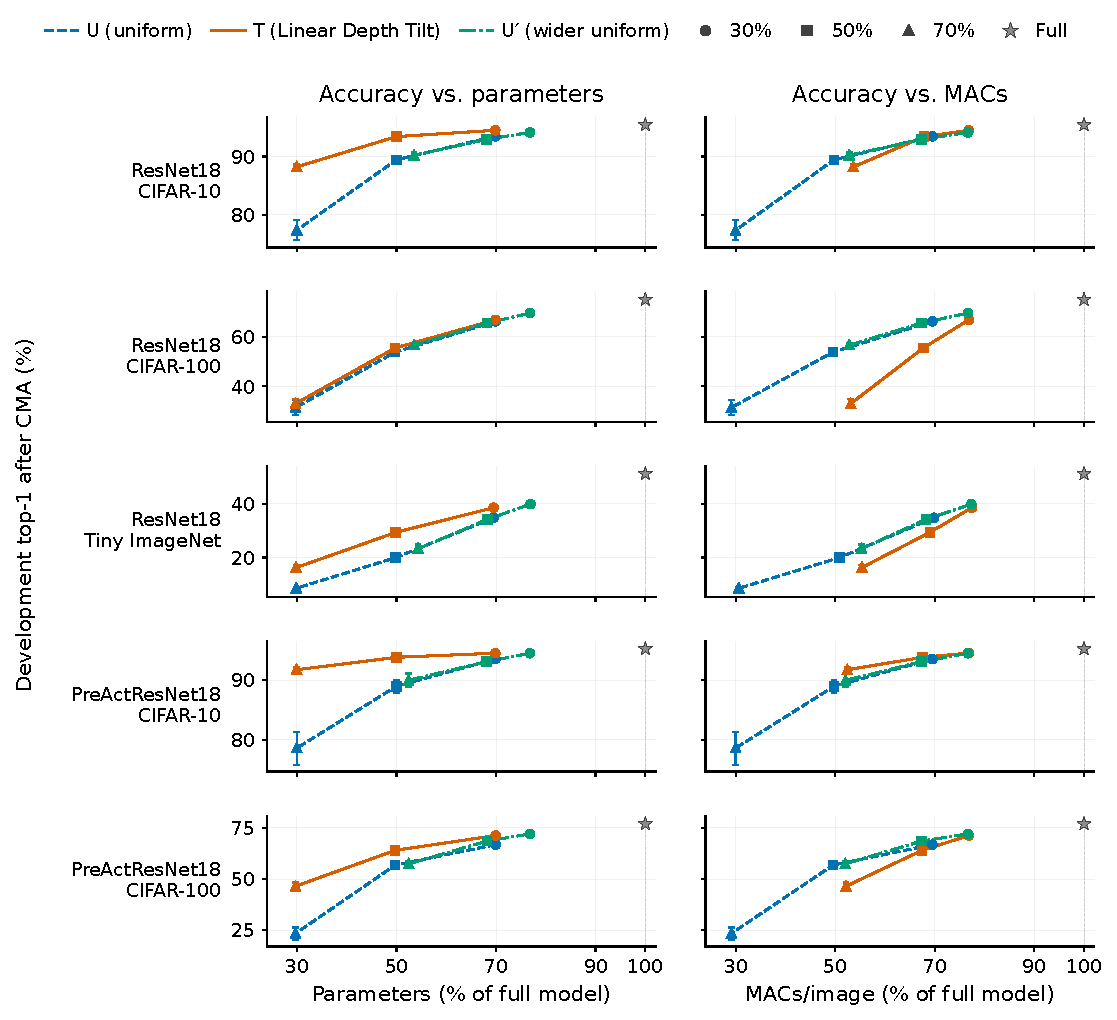
\includegraphics[width=0.89\linewidth]{../experiments/2026-11-08_E037_kontrola_mac/figures/publikacja/e037_accuracy_cost_en.pdf}
  \caption{\textbf{Accuracy and costs on common development data (E037).}
  The wider uniform baseline \Uprime{} wins in 10 of 15 settings at
  comparable MACs and has more parameters. The two columns plot the same
  CMA top-1 results against actual parameters (left) and MACs per image
  (right), as percentages of full-model costs. Markers denote the nominal
  cuts for $U$ and $T$ and associated MAC targets for \Uprime{}. Points and
  bars are means and sample SD across four checkpoints. Top-1 scales are
  shared within a row and vary across rows.}
  \label{fig:comparable-macs}
\end{figure}
% Generated from the audited runs by paper/prepare_tables.py.
\begin{table}[tbp]
\centering
\small
\setlength{\tabcolsep}{3.5pt}
\caption{\textbf{Cost and accuracy on development data.} Top-1 uses the same development split and CMA protocol for uniform folding ($U$), \TiltName{} ($T$), and the wider uniform model $U'$. The anchor is the nominal parameter reduction of $U$ and $T$, not of $U'$. The $U'-T$ column is the mean paired difference; positive values favor $U'$. Section~\ref{sec:allocation-cost} summarizes forward-pass timing ratios.}
\label{tab:cost-controls}
\begin{tabular}{@{}llrrrrrrrr@{}}
\toprule
 &  &  & \multicolumn{3}{c}{Top-1 (\%)} &  & \multicolumn{3}{c}{Cost ratios} \\
\cmidrule(lr){4-6}\cmidrule(lr){8-10}
Architecture & Dataset & Anchor & $U$ & $T$ & $U'$ & $U'-T$ (pp) & \shortstack{MACs\\$T/U$} & \shortstack{Params.\\$U'/T$} & \shortstack{MACs\\$U'/T$} \\
\midrule
ResNet18 & CIFAR-10 & 30\% & 93.495 & 94.520 & 94.155 & $-0.365$ & 1.105 & 1.100 & 0.998 \\
 &  & 50\% & 89.435 & 93.430 & 92.955 & $-0.475$ & 1.364 & 1.363 & 0.992 \\
 &  & 70\% & 77.305 & 88.215 & 90.225 & $+2.010$ & 1.789 & 1.788 & 0.985 \\
\addlinespace[2pt]
ResNet18 & CIFAR-100 & 30\% & 66.340 & 66.960 & 69.670 & $+2.710$ & 1.105 & 1.100 & 0.998 \\
 &  & 50\% & 53.855 & 55.550 & 65.660 & $+10.110$ & 1.366 & 1.371 & 0.994 \\
 &  & 70\% & 31.400 & 33.020 & 56.710 & $+23.690$ & 1.823 & 1.804 & 0.995 \\
\addlinespace[2pt]
ResNet18 & Tiny ImageNet & 30\% & 34.807 & 38.587 & 39.913 & $+1.325$ & 1.109 & 1.106 & 0.998 \\
 &  & 50\% & 19.925 & 29.333 & 34.170 & $+4.837$ & 1.357 & 1.369 & 0.988 \\
 &  & 70\% & 8.433 & 16.180 & 23.240 & $+7.060$ & 1.806 & 1.821 & 0.999 \\
\addlinespace[2pt]
PreActResNet18 & CIFAR-10 & 30\% & 93.590 & 94.575 & 94.550 & $-0.025$ & 1.105 & 1.099 & 0.998 \\
 &  & 50\% & 88.995 & 93.875 & 93.135 & $-0.740$ & 1.358 & 1.363 & 0.996 \\
 &  & 70\% & 78.595 & 91.785 & 90.000 & $-1.785$ & 1.748 & 1.750 & 0.993 \\
\addlinespace[2pt]
PreActResNet18 & CIFAR-100 & 30\% & 66.870 & 71.305 & 72.120 & $+0.815$ & 1.105 & 1.099 & 0.998 \\
 &  & 50\% & 56.845 & 64.070 & 68.585 & $+4.515$ & 1.361 & 1.371 & 0.998 \\
 &  & 70\% & 23.425 & 46.520 & 57.460 & $+10.940$ & 1.790 & 1.766 & 0.998 \\
\bottomrule
\end{tabular}
\end{table}

\FloatBarrier

\paragraph{Matching both costs to \Tilt{} (E041).}
The four controls for ResNet18 at \bfifty{} start from fixed permutations
of earlier \Tilt{} width deviations. We solve a least-squares projection
in the retained fractions $k_g/n_g$ by sequential least-squares
programming, targeting $P=0.9995 C_P$ and $M=0.9995 C_M$ for cost caps
$(C_P,C_M)$. After rounding to integer widths, we deterministically
correct at most two groups if necessary. Both counts must spend
99.9--100\% of the respective caps without exceeding them. The caps are
$P(T)$ and $M(T)$ for E041; the objective uses only geometry. The
projected profiles are adjusted rather than exact permutations.

On CIFAR-100 development data, $T$ exceeds the mean of the four
alternative profiles by 2.10375 pp (4/4) and the best of their means by
0.8600 pp (Table~\ref{tab:dual-tilt}). On CIFAR-10 the advantage over
their mean is 0.11250 pp (2/4), and control~104 beats $T$ by 0.3850 pp,
with gains on all four checkpoints. The study's criterion of a positive
mean with at least three positive pairs on each dataset is not met.
Tiny ImageNet is outside this pilot's scope.

% Generated from the audited runs by paper/prepare_tables.py.
\begin{table}[tbp]
\centering
\small
\setlength{\tabcolsep}{5pt}
\caption{\textbf{Both costs matched to \Tilt{}.} Four prespecified ResNet18 controls at the nominal 50\% parameter cut, each using 99.9--100\% of \Tilt{}'s parameters and MACs. $\bar C$ is the mean of the four controls within each checkpoint. The positive count refers to $T-\bar C$. The best control is identified descriptively by mean development top-1.}
\label{tab:dual-tilt}
\begin{tabular}{@{}lrrrrrr@{}}
\toprule
 & \multicolumn{2}{c}{Top-1 (\%)} &  &  &  &  \\
\cmidrule(lr){2-3}
Dataset & $T$ & $\bar C$ & $T-\bar C$ (pp) & Positive & Best control & $T-$best (pp) \\
\midrule
CIFAR-10 & 93.4300 & 93.31750 & $+0.11250\pm 0.2184$ & 2/4 & 104 & $-0.3850$ \\
CIFAR-100 & 55.5500 & 53.44625 & $+2.10375\pm 0.7602$ & 4/4 & 103 & $+0.8600$ \\
\bottomrule
\end{tabular}
\end{table}

\FloatBarrier

\section{Mild cuts on development data}
\label{app:mild}

\paragraph{Matched parameter counts (E051).}
At nominal 5\% and 10\% cuts, we choose the largest common retention for
$U$ under the parameter cap on the integer grid. We fit the linear profile
with $\alpha=0.30$ against $P(U)$ using the lower bound $r_g\ge 0$ and
adjust widths if needed to match $P(U)$ to within 0.1\%. Both budgets
were fixed before scoring. Each dataset uses the same A4096/CMA across
profiles; on Tiny the minimum crop area fraction is 0.65
(Appendix~\ref{app:offsets}). The b10 targets for this diagnostic are at
least 9.5\% parameter reduction, mean gain of at least 1 pp over $U$ with
at least three positive pairs, and mean loss to the full model of at most
3 pp. CIFAR-100 meets all targets; Tiny has a 3.6075 pp mean loss. At b10,
the linear profile reduces parameters by about 10.4\% and MACs by 3.35\%
relative to the corresponding full model. The 5\% cut is descriptive:
Tiny achieves 61.3250\%, with a loss of 1.2875 pp and about 1.69\% fewer
MACs than the full model. Table~\ref{tab:tilt-mild-dev} reports both cuts.

% Generated from the audited runs by paper/prepare_tables.py.
\begin{table}[tbp]
\centering
\small
\setlength{\tabcolsep}{5pt}
\caption{\textbf{Mild cuts at matched parameter counts (development diagnostic).} $T$ uses 99.9--100\% of $U$'s parameters; MACs are reported rather than capped. Mean top-1 after the same BN procedure within each dataset; all differences favor $T$ on all four checkpoints. Parameter and MAC reductions are calculated relative to the full model.}
\label{tab:tilt-mild-dev}
\begin{tabular}{@{}lrrrrrrr@{}}
\toprule
 & \multicolumn{2}{c}{Top-1 (\%)} &  &  & \multicolumn{2}{c}{Reductions for $T$ (\%)} &  \\
\cmidrule(lr){2-3}\cmidrule(lr){6-7}
Nominal $P$ cut & $U$ & $T$ & $T-U$ (pp) & $T$ loss (pp) & $P$ & MACs & $M(T)/M(U)$ \\
\midrule
\multicolumn{8}{@{}l}{\textbf{CIFAR-100 (full top-1 80.9700\%)}} \\
\addlinespace[2pt]
10\% & 77.9850 & 79.7500 & $+1.7650$ & 1.2200 & 10.41 & 3.35 & 1.086 \\
5\% & 79.5600 & 80.4250 & $+0.8650$ & 0.5450 & 5.25 & 1.69 & 1.043 \\
\midrule
\multicolumn{8}{@{}l}{\textbf{Tiny ImageNet (full top-1 62.6125\%)}} \\
\addlinespace[2pt]
10\% & 57.2925 & 59.0050 & $+1.7125$ & 3.6075 & 10.40 & 3.35 & 1.086 \\
5\% & 60.2125 & 61.3250 & $+1.1125$ & 1.2875 & 5.24 & 1.69 & 1.043 \\
\bottomrule
\end{tabular}
\end{table}


\paragraph{Local width redistribution at 10\% (E052).}
Six profiles shift width from two stage-3 hidden groups to stage 4,
reduce parameters by at least 9.5\%, match $P(U)$ to within 0.1\%, and
respect the parameter and MAC caps of the b10 linear profile. With the
E051 operator and calibration, we
select a single profile per dataset by mean negative log-likelihood over
four checkpoints on a fixed subset of 8,000 training images disjoint from
calibration and development. The same profile (S04) is selected on both
datasets and is the only new profile evaluated on development data. It
reduces both stage-3 hidden widths from 256 to 243 and increases the
stage-4 output width from 474 to 482 relative to $T$. Top-1 is 79.8850\%
on CIFAR-100 ($+0.1350$ pp over $T$, 2/4) and 59.2050\% on Tiny ImageNet
($+0.2000$ pp, 3/4), with 0.94\% fewer MACs than $T$ on both datasets.
The Tiny loss of 3.4075 pp remains above the prespecified 3 pp target for
this experiment.
\FloatBarrier

\section{Frozen width offsets under joint caps}
\label{app:offsets}

\paragraph{Selection and transfer (E042).}
At \bfifty{}, we form 24 feasible profiles per dataset before scoring:
eight within-stage exchanges, four across-stage exchanges, and twelve
proposals with random offsets in retention fractions. We use the
projection described in Appendix~\ref{app:costs} with caps $P(U)$ and
$M(U)$. The width domain is
$\lfloor 0.1 n_g\rfloor\le k_g\le\lfloor 0.9 n_g\rfloor$; both counts
must be within 0.1\% of their caps from below. We select one candidate by
mean post-CMA top-1 over the four checkpoints on labeled CIFAR-100
development data. The selected random-offset proposal (L06) is the
\emph{\FrozenProfile{}}, labeled \emph{\FrozenShort{}} in tables. It gains
1.175 pp (3/4) over $U$ on the selection split; five candidates beat $U$
on average and the median
contrast is $-1.265$ pp. CIFAR-10 serves as a control and does not select
L06. Uniform folding and $T$ projected onto the same caps ($T_{\rm proj}$)
are separate references.

We freeze the proposed offsets in retention fractions, in percentage
points in upstream group order:
\[
 \mathbf o=(+2,-15,-14,+13,-1,-5,-6,+9,-12,-13,+17,-6).
\]
At a new budget, we add $n_g o_g/100$ to the realized uniform width
$k_g^U$, round to nearest (ties to even), clip to the legal range, and
project to the two caps. Thus the offsets stay fixed and the integer
widths are fitted to the architecture and costs. At \bfifty{} on the
CIFAR-100 reserve we reuse the selected widths exactly. At \bten{}, $U$
has the largest common retention under $P(U)\le\lfloor 0.9P(\mathbf n)\rfloor$.
We allow $k_g\le n_g$ so that uncut groups are possible. The earlier
upper bound would require at least a 19.21\% parameter cut on the older
Tiny model. To form the mild $T_{\rm proj}$ proposal, we first fit the
linear profile at $\alpha=0.30$ with $r_g\ge 0$ under $P(U)$, then apply
the same joint projection. The resulting $T_{\rm proj}$ and frozen
offsets spend 99.9--100\% of both caps.

\paragraph{New checkpoints at b10 (E049).}
The held-out images are the previously used official splits, and the
offsets, geometries, and evaluation targets are fixed before scoring the
new folded models. All three folded profiles save 10.36--10.41\% of
parameters and 10.97--11.06\% of MACs from their respective full models.
The frozen-offset profile improves over $U$ by 0.6150 pp on CIFAR-100
and 0.6750 pp on Tiny (sample SD 0.4487 and 0.4970 pp), and over $T_{\rm proj}$ by
0.6700 and 1.8000 pp, respectively, with four positive pairs in each
comparison. On Tiny, $T_{\rm proj}$ trails $U$ by 1.1250 pp. Mean losses
to the full model for frozen offsets are 1.6575 and 4.5700 pp
(Table~\ref{tab:b10-transfer}). The prespecified targets here are at
least 9.5\% reductions in both counts, a mean gain of at least 1 pp over
$U$ with at least three positive pairs, and a loss of at most 3 pp. The
mean gains fall short on both datasets, and the loss exceeds the target
on Tiny.

% Generated from the audited runs by paper/prepare_tables.py.
\begin{table}[tbp]
\centering
\small
\setlength{\tabcolsep}{7pt}
\caption{\textbf{Nominal 10\% parameter cut under both UNIFORM budgets on newly trained ResNet18 models.} Each pair starts from the same checkpoint and uses the same BN recalibration, including the full-model reference. Top-1 and loss are means across four checkpoints on 10,000 images per dataset. Projected TILT adjusts the linear profile to both budgets. The official test and validation splits had previously been evaluated in this project.}
\label{tab:b10-transfer}
\begin{tabular}{@{}lrrrr@{}}
\toprule
Model & Top-1 (\%) & Loss to full (pp) & Parameters & MACs/image \\
\midrule
\multicolumn{5}{@{}l}{\textbf{CIFAR-100 (official test)}} \\
\addlinespace[2pt]
Full model & 79.6800 & 0.0000 & 11,220,132 & 555,468,800 \\
UNIFORM & 77.4075 & 2.2725 & 10,055,630 & 494,537,444 \\
Projected TILT & 77.3525 & 2.3275 & 10,051,974 & 494,077,516 \\
Frozen offsets & \textbf{78.0225} & 1.6575 & 10,052,748 & 494,053,376 \\
\midrule
\multicolumn{5}{@{}l}{\textbf{Tiny ImageNet (official validation)}} \\
\addlinespace[2pt]
Full model & 61.2175 & 0.0000 & 11,271,432 & 555,520,000 \\
UNIFORM & 55.9725 & 5.2450 & 10,104,230 & 494,585,944 \\
Projected TILT & 54.8475 & 6.3700 & 10,100,626 & 494,294,552 \\
Frozen offsets & \textbf{56.6475} & 4.5700 & 10,104,048 & 494,104,576 \\
\bottomrule
\end{tabular}
\end{table}


\paragraph{Sensitivity to Tiny calibration (E050).}
On development data we increase the minimum random crop area fraction
for BN recalibration from 0.40 to 0.65, the value used to train the new
Tiny models. Indices, crop and flip seeds, CMA, weights, and widths stay
fixed. Top-1 rises by 0.9250 pp for the full model, 1.1275 pp for $U$,
1.4500 pp for $T_{\rm proj}$ and 1.3200 pp for frozen offsets (4/4 for
each). The mean gain of frozen offsets over $U$ changes from 0.7250 to
0.9175 pp (3/4 under either crop), and its loss to the full model falls
from 4.7975 to 4.4025 pp. We do not evaluate this crop change on the
official benchmark.
\FloatBarrier

\paragraph{Transfer on earlier checkpoints (E043--E047).}
On a separate 5,000-image CIFAR-100 reserve, held out before training
and profile selection, L06 gains 1.215 pp (3/4) at \bfifty{} over $U$
and 1.065 pp (4/4) over $T_{\rm proj}$. Its gain at \bthirty{} over $U$
is 0.945 pp (4/4), below the prespecified 1 pp target. Corresponding
losses to the full model are 19.970 and 7.420 pp. On the previously used
official Tiny validation set (not used to select L06), the transferred
profile gains 2.100 pp (4/4) at \bfifty{} and 0.255 pp (3/4) at
\bthirty{} over $U$; the \bfifty{} gap to the full model is 29.0375 pp.

At \bten{} on the earlier Tiny model, the frozen-offset profile uses
\[
 \mathbf k=(64,52,53,128,127,119,233,256,219,434,512,476).
\]
It uses 6,575 fewer parameters and 34,004 fewer MACs per image than
$U$. We reproduce
the eight full and uniform states and scores from the earlier Tiny
development run, and observe a 1.1425 pp gain for frozen offsets (4/4,
sample SD 0.8820 pp). The loss to full falls from 4.8575 to 3.7150 pp.
By comparison, uniform folding at a separate 20\% cut loses 10.6400 pp
on this split.

We also evaluate these widths on the ImageNetV2 MatchedFrequency sample
\texttt{imagenetv2-b-33} \citep{recht2019imagenetv2}, restricted to the
200 Tiny classes (2,000 images, ten per class). Label mapping is checked
against release metadata; exact RGB and perceptual hash screening against
110,000 Tiny training, development, and official validation images flags
no duplicates. We resize the
whole RGB image bilinearly to $64\times64$ after EXIF orientation and
apply the Tiny normalization without augmentation. Before scoring we
verify that the 12 post-CMA states and costs match those from the Tiny
development run. BN uses Tiny training images without adapting to
ImageNetV2. Frozen offsets gains 1.3500 pp (4/4, sample SD 0.9704 pp)
over $U$ and reduces the loss to the full model from 3.35 to 2.00 pp
(Table~\ref{tab:b10}).

% Generated from the audited runs by paper/prepare_tables.py.
\begin{table}[tbp]
\centering
\small
\setlength{\tabcolsep}{8pt}
\caption{\textbf{Mild compression under both uniform-folding caps.} Cost counts are identical across samples. For each checkpoint, top-1 loss is the full model's top-1 minus that of the specified model on the same images. Values are mean $\pm$ sample SD across four checkpoints after CMA. The ImageNetV2 sample is MatchedFrequency restricted to the 200 Tiny ImageNet classes.}
\label{tab:b10}
\begin{tabular}{@{}lrrrr@{}}
\toprule
Model & Parameters & MACs/image & Top-1 (\%) & Paired loss (pp) \\
\midrule
\multicolumn{5}{@{}l}{\textbf{Tiny ImageNet development split (10,000 images)}} \\
\addlinespace[2pt]
Full model & 11,279,112 & 148,148,224 & $51.2200\pm 0.1602$ & 0 \\
Uniform folding & 10,111,430 & 132,336,196 & $46.3625\pm 0.4687$ & $4.8575\pm 0.5309$ \\
Frozen Offset Profile & 10,104,855 & 132,302,192 & $47.5050\pm 0.4458$ & $3.7150\pm 0.5132$ \\
\midrule
\multicolumn{5}{@{}l}{\textbf{ImageNetV2 (2,000 images)}} \\
\addlinespace[2pt]
Full model & 11,279,112 & 148,148,224 & $30.3375\pm 0.3198$ & 0 \\
Uniform folding & 10,111,430 & 132,336,196 & $26.9875\pm 1.0711$ & $3.3500\pm 0.7853$ \\
Frozen Offset Profile & 10,104,855 & 132,302,192 & $28.3375\pm 0.2496$ & $2.0000\pm 0.2483$ \\
\bottomrule
\end{tabular}
\end{table}


For the ImageNetV2 comparison and the frozen-offset comparison at
\bfifty{} on Tiny validation, we estimate paired 95\% percentile
intervals by 10,000 bootstrap draws, resampling images within each class
with the same resampled indices for all variants and checkpoints. The
intervals are $[+0.700,+2.025]$ pp on ImageNetV2 and $[+1.67,+2.52]$ pp
for \bfifty{} on Tiny validation. The former meets the prespecified
criterion (positive mean, at least three positive pairs, positive lower
interval limit). Both intervals describe variation across sampled images
conditional on the four fixed checkpoints; the external image sample
does not add training replicates or extend the class set. Its absolute
scores reflect a different image source and preprocessing.
\FloatBarrier
